\documentclass{article}
\usepackage[utf8]{inputenc}
\usepackage[margin=3cm]{geometry}
\title{CSEN 901: Introduction to Artificial Intelligence \\Projct 1: Water Sort}
\author{Project Report \vspace{24pt} \\ Abdelrahman Aboelkehir, Hossain Ghoraba, \\ Mahmoud Aboelenein, Omar Hesham}
\date{18.10.2024}


\usepackage{natbib}
\usepackage{graphicx}
\usepackage{dirtree}
\usepackage{algorithm}
\usepackage{algpseudocode}

\begin{document}

\maketitle

\section{Introduction}
This project is the implementation of a search agent to solve the water sort puzzle. You can find a description of the water sort puzzle in the document titled \textbf{Project Description.pdf}. The agent is implemented in Java. The search the agent performs does not prune any branches early, nor does it perform any checks for whether the current node can or can not lead to a solution. A branch in the search is terminated only when there are no more possible nodes to expand from the leaf of that branch (in this probelm, this means there are no possible pour combinations to apply to the current state). The search terminates when either \textbf{a.} A node selected for expansion is identified as a goal state, or \textbf{b.} No more nodes on the search frontier can be expanded.

\newpage

\section{Project Hierarchy}

Here is a hierarchy of all the project files:

\dirtree{%
.1 src.
.2 main.
.3 java.
.4 code.
.4 generic.
.5 QueueingFunctions.
.6 QueueingFunction <<Interface>>.
.6 AStar1QueueingFunction.
.6 AStar2QueueingFunction.
.6 EnqueueAtEnd.
.6 EnqueueAtFront.
.6 EnqueueAtFrontWithDepthLimit.
.6 GREEDY1QueueingFunction.
.6 GREEDY2QueueingFunction.
.5 FixedSizeStack.
.5 Operator <<Interface>>.
.5 OperatorResult.
.5 Problem.
.5 SearchState.
.6 OrderedInsert.
.4 utils.
.5 ConditionalPrintStream.
.5 Methods.
.5 WaterSortUtils.
.4 watersort.
.5 Bottle.
.5 Color.
.5 LayerGroup.
.5 Pour.
.5 WaterSortProblem.
.5 WaterSortState.
.5 WaterSortUtils.
.4 GenericSearch.
.4 Node.
.4 WaterSortSearch.
}

\newpage

\begin{figure}[t]
\section{Class Diagram}
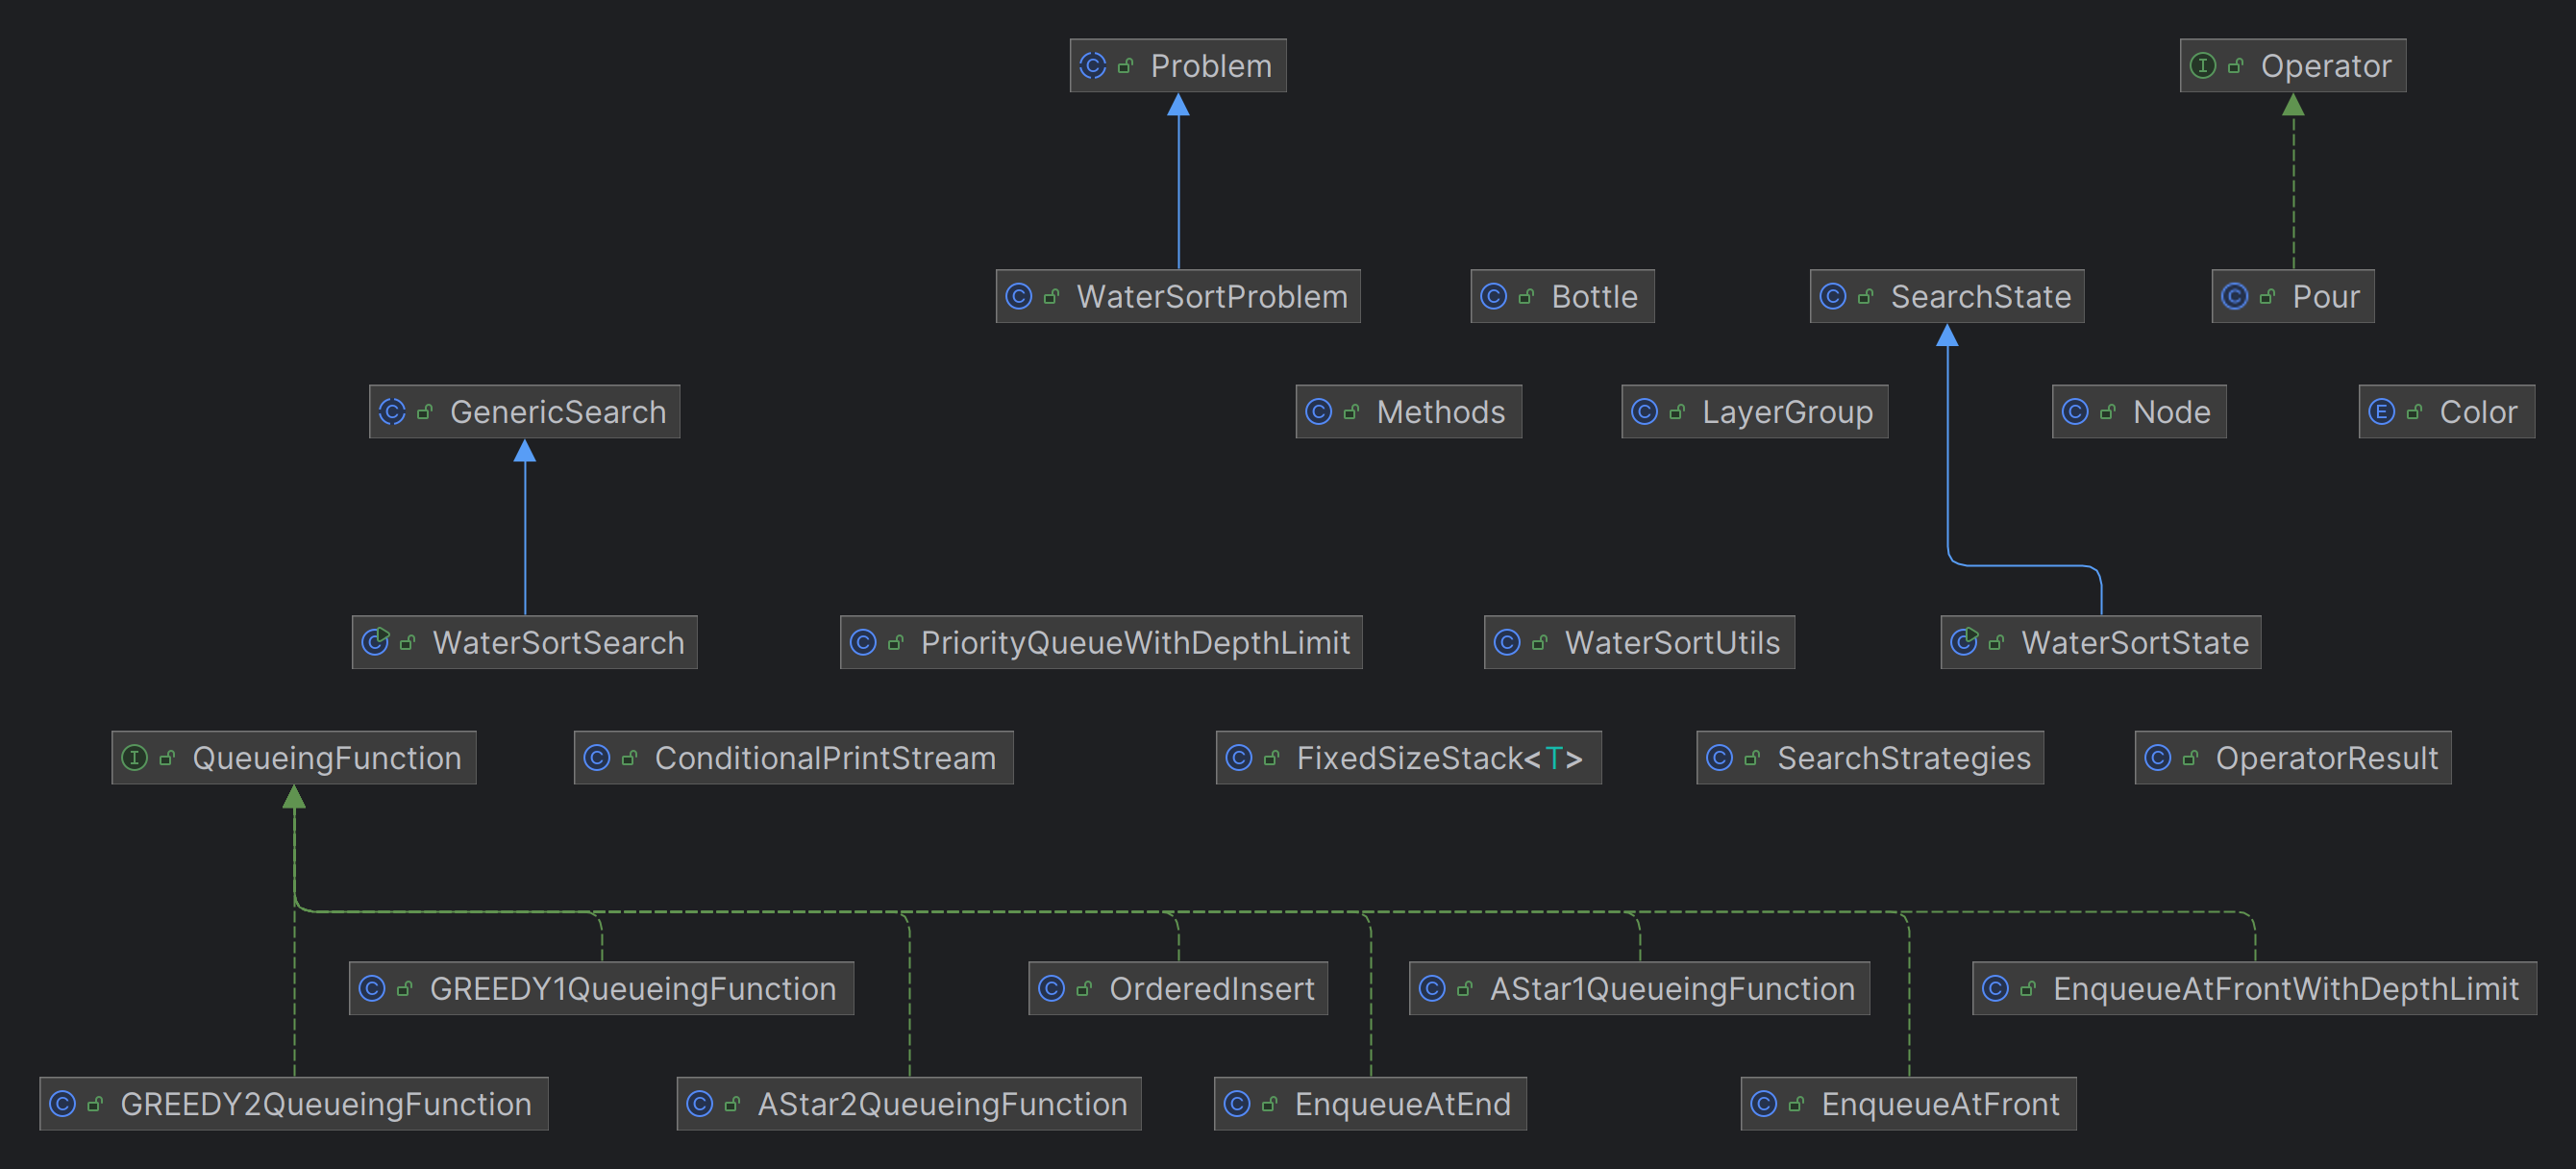
\includegraphics[scale=0.18]{Class Diagram.png}
\caption{Class Diagram}
\end{figure}

\section{Implementation of the Search Algorithms}

Our implementation for all search algorithms closely follows the description of the \textsl{GeneralSearch} algorithm outlined in lecture 2 of the course: 


\begin{algorithm}
\caption{GENERAL-SEARCH(problem, QING-FUN)}
\begin{algorithmic}[1]
    \State \textbf{return} a solution, or failure
    \State $nodes \gets \texttt{MAKE\_Q}(\texttt{MAKE\_NODE}(\texttt{INIT\_STATE}(problem)))$
    \While{true}
        \If{$nodes is empty$}
            \State \textbf{return} failure
        \EndIf
        \State $node \gets \texttt{REMOVE\_FRONT}(nodes)$
        \If{$\texttt{GOAL\_TEST}(problem)(\texttt{STATE}(node))$}
            \State \textbf{return} node
        \EndIf
        \State $nodes \gets \texttt{QING\_FUN}(nodes, \texttt{EXPAND}(node, \texttt{OPER}(problem)))$
    \EndWhile
\end{algorithmic}
\end{algorithm}

All the algorithms use a Java \texttt{PriorityQueue} as their queue. The \texttt{PriorityQueue} in Java orders objects based on a given \texttt{Comparator}. The classes in the \texttt{QueueingFunctions} package create and return a \texttt{PriorityQueue} with the appropriate \texttt{Comparator}, which will then be used to hold and order all the nodes during the search. \\

\newpage

For example, here is the queuing function for Breadth-First Search: 

\begin{verbatim}
public class EnqueueAtEnd implements QueuingFunction {
  @Override
  public PriorityQueue<Node> apply() {
    return new PriorityQueue<>(Comparator.comparingInt(Node::getDepth));
  }
}
\end{verbatim}

In this case, a \texttt{PriorityQueue} is created using a comparator that says to order the nodes by depth in ascending order. Consequently, all the nodes in this queue will be ordered in ascending order of depth. \\

Here is a comprehensive list of the way by which the \texttt{PriorityQueue} orders nodes within it for every search algorithm we have implemented:

\begin{enumerate}
\item Breadth-First Search (BFS): Depth (ascending, i.e from \textit{shallowest} to \textit{deepest})
\item Depth-First Search (DFS): Depth (descending, i.e from \textit{deepest} to \textit{shallowest})
\item Iterative Deepening Depth-First Search (IDS): Same as DFS
\item Uniform-Cost Search (UCS): Path cost from the root to the node \texttt{(f(n) = g(n))}(ascending)
\item Greedy Best-First Search: The value of the heuristic function \texttt{(f(n) = h(n))}(we have two \textbf{admissible} heuristics we can use)
\item A* Search: The value of the path from the root plus the heuristic value for the current node (\texttt{f(n) = g(n) + h(n)})
\end{enumerate}

\newpage

Here is the main body of how searching is done (in the \texttt{GenericSearch} class):
\begin{verbatim}
public static Node generalSearch(Problem problem, QueuingFunction queuingFunction, boolean visualize)
            throws CloneNotSupportedException {
        nodesExpanded = 0;
        int nodesVisited = 0;
        Node solutionNode = null;
        expandedStates.clear();
        candidateSolutions.clear();

        Node initialNode = makeNode(problem.getInitialState());
        PriorityQueue<Node> nodes = queuingFunction.apply();
        nodes.add(initialNode);

        while (!nodes.isEmpty()) {
            Node currentNode = removeFront(nodes);
            currentNode.setOrderOfVisiting(nodesVisited++);
            if (problem.goalTestFn(currentNode)) {
                solutionNode = currentNode;
                break;
            }
            List<Node> expandedNodes = expand(currentNode, problem.getOperators(), problem);
            nodes.addAll(expandedNodes);
        }

        return solutionNode;
    }
\end{verbatim}

\subsubsection{Goal Test}
One important thing to mention is that the goal test is applied to a node first when it is selected for expansion, not when it is created. This has the unfortunate side-effect of increasing the time complexity of DFS from $O(b^{d})$ to $O(b^{d+1})$, because an extra level (at least in the worst case) will be created beyond the goal node before the goal node is selected for expansion and discovered to be a goal, as well as perhaps increasing the time complexity of the rest of the search algorithms (by a factor I am not sure I can calculate), but has the fortunate side-effect of making UCS optimal (if the goal test was applied to a node when it is first created, UCS would not be optimal). If you are curious, you can find a small discussion of why this may be the case in Russel \& Norvig, section 3.4.2

\subsection{Heuristic Functions}

We have mentioned earlier that we have two heuristic functions available for use. In this section, we will examine those two heuristic functions and argue why they may be admissible. \\

\textbf{Heuristic 1: } The number of bottles where the layers are not all the same color

It is easy to show that this heuristic is admissible. For any state not to be a goal state, there must be at least 1 bottle where all the layers are not the same color. To make this state a goal state, you must pour at least 1 layer from one bottle to another. Therefore, this heuristic can never overestimate the cost (which is the number of layers poured) of the solution. \\

\newpage

\textbf{Heuristic 2: } The difference between the current filled capacity of the bottle and the highest number of layers with the same color, all added up together.

For example, consider the following state with 3 bottles: \texttt{[e,e,r,g,r], [b,r,b,b,y], [e,e,e,e,e]}. The value of the heuristic function for this state will be: $(5 - 2) + (5 - 3) + (0) = 5$ \\

It is also not too difficult to show that this heuristic is admissible. If the node is a goal state (either all the bottles are empty, or all the bottles have layers of the same color), its value is 0. For a state that is only one layer away from a goal state, such as \texttt{[y,y,y,y,y], [b,b,b,g], [g,g,g,g]}, the value of the heuristic is $(0) + (1) + (0) = 1$. And this is in the "best-case" scenario where the layer to be poured is directly on top. If the layer(s) was/were anywhere other than on top, it would certainly take more than 1 pour operation to reach a goal state. Notice that we only calculate the difference between the filled capacity of the bottle and the number of the most repeated color layer. \\

The value of this heuristic for an empty bottle is therefore 0 (current capacity: 0 - number of most repeated color: 0, = 0.)

\subsection{Implementation of Iterative-Deepening Depth-First Search}

IDS is special in that it is the only search algorithm that works differently from the remaining search algorithms. For the remaining search algorithms, nodes are simply added to the \texttt{PriorityQueue}, removed from the front of the queue, and expanded, until either the queue is empty (there are no more nodes left to expand), or a solution node has been found. IDS works differently because when it reaches its depth limit, it increases the depth limit by 1 and reruns DFS from the initial state using the increased depth limit. In this section, we would like to discuss some of the implementation details regarding our implementation of IDS. \\

\textbf{ >>> CONTINUE HERE <<<}
\end{document}